\chapter{Evaluation}

In this chapter, we present the results for various models on three datasets. First, we provide a description and origin of these datasets. Then we compare the performance of the models and the datasets. This includes comparison of open source data downloaded from the Internet with the proprietary data provided by the private company. In the third section, we compare the performance for different number of recommendations.\todo{What else? There should probably be more.}

\section{Datasets}

To evaluate performance of a model, a set of necessary data is necessary. We provide description of the three datasets that we chose for the evaluation of the models in this section.

\subsection{Firefox Data}

This dataset is downloaded from Mozilla repository\footnote{https://bugzilla.mozilla.org} in product Firefox. We downloaded all bugs that are in status \texttt{RESOLVED} with resolution \texttt{FIXED} and were created in year 2010 or later. We also removed bugs with field \texttt{assigned\_to} set to \texttt{nobody@mozilla.org} as those tickets were resolved and fixed but not assigned. This yields $9,141$ bugs in total. To get a better comparison with the other datasets, we only use $3,000$ datasets for training and cross-validation that were created between 2010-01-01 and 2012-07-10. This dataset contains $343$ labels (developers). Finally, we remove developers who did not fix at least $30$ bugs, yielding $1,810$ bugs with $20$ developers. The histogram with frequencies of the developers and cumulative distribution is on figure~\ref{fig:datasets.firefox.dist}.

\begin{figure}[htbp]
    \centering
        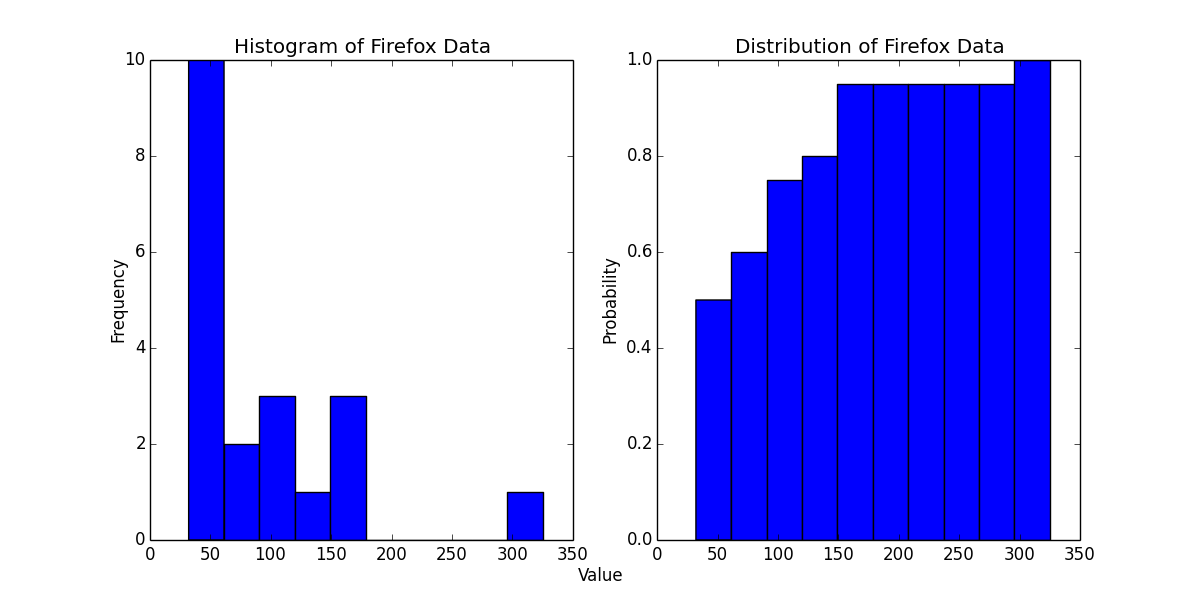
\includegraphics[width=\textwidth]{./images/distribution/firefox.png}
    \caption{Histogram and distribution of the Firefox data.}
    \label{fig:datasets.firefox.dist}
\end{figure}

\subsection{Netbeans Data}

Netbeans data were downloaded from Netbeans bug repository\footnote{https://netbeans.org/bugzilla/}. We considered latest $3,000$ bugs that are in status \texttt{RESOLVED} with resolution \texttt{FIXED}. We removed bugs with assignee \texttt{kenai\_tester\_git} as those were created automatically resulting in $2,924$ bug reports. These bugs were created between 2014-06-14 and 2015-06-14 and they contain $92$ developers. After removing developers who did not fix at least 30 bugs, the dataset contains $2,528$ reports with $30$ developers. Figure~\ref{fix:datasets.netbeans.dist} is a histogram and distribution of this datasets.

\begin{figure}[htbp]
    \centering
        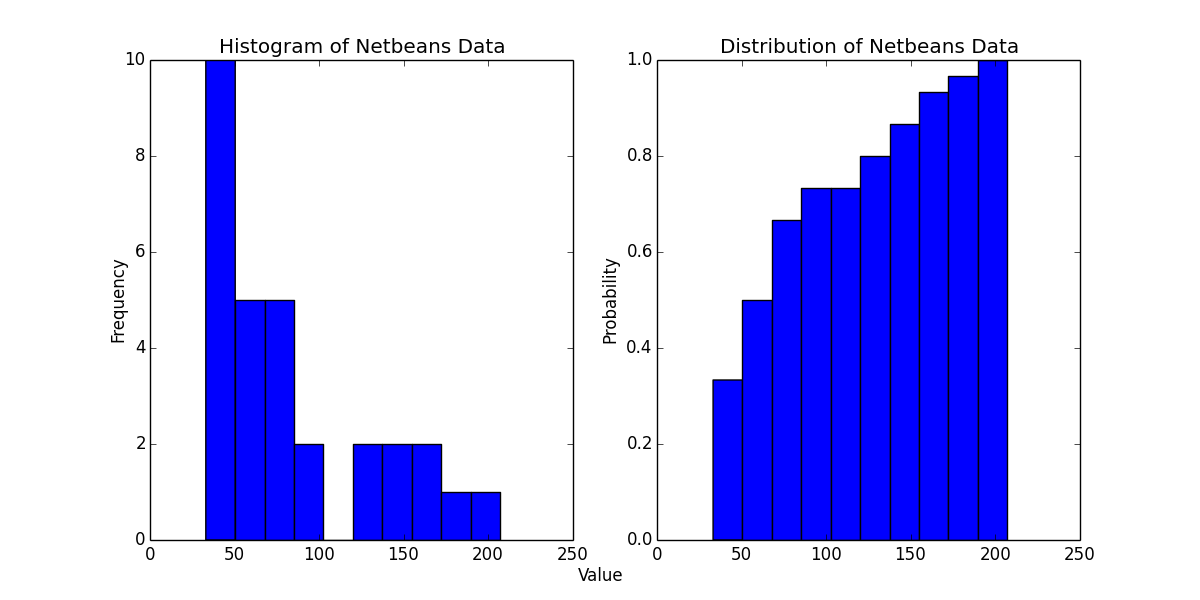
\includegraphics[width=\textwidth]{./images/distribution/netbeans.png}
    \caption{Histogram and distribution of the Netbeans data.}
    \label{fig:datasets.netbeans.dist}
\end{figure}

\subsection{Proprietary Data}

The Proprietary dataset was provided by a company that wants to remain anonymous. The provided dataset contains $2,243$ bug reports created between 2009-03-07 and 2013-08-23. Only bug reports that were resolved with assigned developer were considered. There are $141$ developers in this dataset. Only $1,479$ bugs assigned to $28$ developers were retained after removal of developers with less than $30$ fixed bugs. The histogram and probability distribution is pictured on figure~\ref{fig:datasets.proprietary.dist}.

\begin{figure}[htbp]
    \centering
        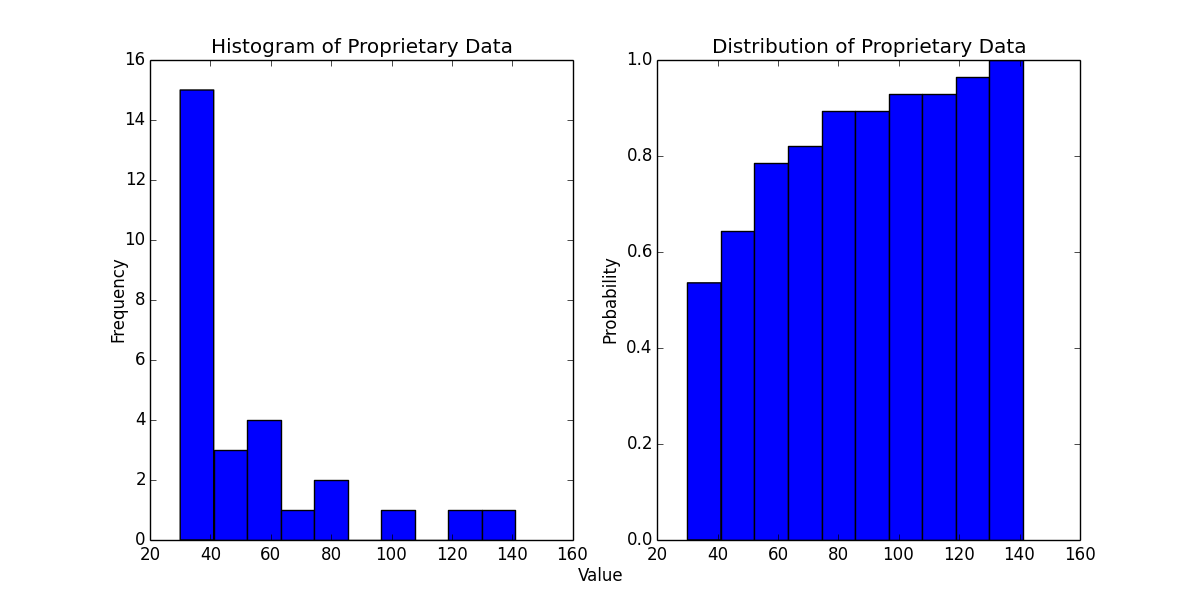
\includegraphics[width=\textwidth]{./images/distribution/proprietary.png}
    \caption{Histogram and distribution of the Proprietary data.}
    \label{fig:datasets.proprietary.dist}
\end{figure}

\subsection{Chi-Squared Test}

In this section, we test the null hypothesis that two samples are from the same distribution. For this, we use the two-sided alternative of two-sample Chi-Squared test. We split the samples from each datasets into five bins and compute the \textit{p-value} for three pairs of samples (Netbeans and Firefox, Firefox and Proprietary, Proprietary and Netbeans).

The Chi-Squared test with Netbeans and Firefox samples yields p-value of $0.4283$, as p-value~$> 0.05$ we fail to reject the null hypothesis that the two samples are from the same distribution with 5\% level of significance.

The test with Firefox and Proprietary samples returns p-value equal to $0.8169$ so we again fail to reject the null hypothesis with 5\% level of significance. The last test with samples from Proprietary and Netbeans data results in p-value of $0.6735$, which again means the null hypothesis cannot be rejected with 5\% significance level.

\subsection{T-Test}

In the previous section, we tested the hypothesis that the datasets used in this thesis are from the same distribution. We failed to reject the hypothesis with all samples, in this section, we test the null hypothesis that the samples have the same population mean. For that, we have to test the hypothesis that the variance of the samples are the same.

We use the two-sided alternative of the standard independent two-sample t-test to test the null hypothesis that the samples have the same population mean, and the two-sided alternative of the Levene test to test the null hypothesis that the samples have equal population variance. If we reject the null hypothesis of the Levene test, we use the two-sided alternative of the Welch's t-test instead of the standard t-test.

First, we test the samples from Firefox and Proprietary datasets. The Levene test yields p-value equal to $0.0373$, as p-value~$< 0.05$, we reject the null hypothesis with 5\% significance level. To test the population mean of the two samples, we therefore have to use the Welch's t-test. The Welch's t-test results in p-value of $0.0343$, which means we have to reject the null hypothesis of equal population mean of the two samples with 5\% significance.

Second, we test the samples from Firefox and Netbeans repositories. As the Levene tests returns p-value equal to $0.5166$, which is greater than the $\alpha$ of $0.05$, we fail to reject the null hypothesis of equal population variances with 5\% level of significance. Next, we use the standard independent t-test to test the population means. The p-value of this t-test on these two samples is equal to $0.7138$, which means we fail to reject the null hypothesis of equal population means with 5\% significance.

Last samples we test are from Netbeans and Proprietary datasets. The p-value of the Levene test for these two samples is $0.0216$ thus we reject the null hypothesis of equal variances. The p-value of the Welch's t-test is equal to $0.0039$, which again means we can reject the null hypothesis that the two samples have the same population mean with 5\% significance.

\section{Window Size}

The size of the time window is an important question that needs to be addressed when dealing with machine learning. A naive approach uses all samples from a dataset to train the classifier, but a more advanced approach considers what effect does the size of the window have on the data and how it can improve the performance. In this section, we try to address this concern by evaluating the performance of the classifier for different sizes of the window.

To determine weather a different size of the window helps the performance is a difficult endeavour, we attempt it by employing three different approaches, each approach can be described by two properties like this:

\begin{enumerate}
 \item Fixed number of bugs in each period, variable size of the train set
 \item Variable number of bugs in each period, fixed size of the train set
 \item Variable number of bugs in each period, variable size of the train set
\end{enumerate}

The Firefox dataset is used for testing of all approaches. The model that is used is Support Vector Machine with Stop-Words removed and TF-IDF weighing.

\subsection{First Approach}

In the first approach, we first remove all bugs from the whole dataset that were fixed by developers with less than 20 fixed bugs. Then we split the remaining dataset into 8 bins. First bin contains 1000 randomly selected bug reports from period 1. All subsequent bins (2-8) contain 500 randomly selected reports from periods 2-8. There are 8 periods, first period is about one year long, all the other periods are about half a year long each. All periods combined add up to the time span of the whole dataset and each $n+1$ period contains bugs older than $n$ period. We train the classifier on period 1, then 1-2, 1-3, 1-4, 1-5, 1-6, 1-7 and 1-8. We test each trained classifier on the same cross-validation set of 300 bug reports that are newer than bugs in period 1.

The disadvantage of this approach is that you select fixed number of bugs from each period. In real world, each period can contain different number of bug reports based e.g. on season. Another disadvantage is that you remove developers that do not meet the criteria of 20 bugs fixed based on the whole dataset. If some developers were very active in the past but are no longer very relevant, they will not be removed from a dataset that is constructed from periods in which the developer no longer fulfills the criteria.

The result is visualized on figure~\ref{fig:window.firefox.1a}. You can see that about the best result is achieved with the size of the window equal to 30 months. Unfortunately, the performance of the classifier for other sizes is very similar and the results is therefore quite inconclusive.

\begin{figure}[htbp]
    \centering
        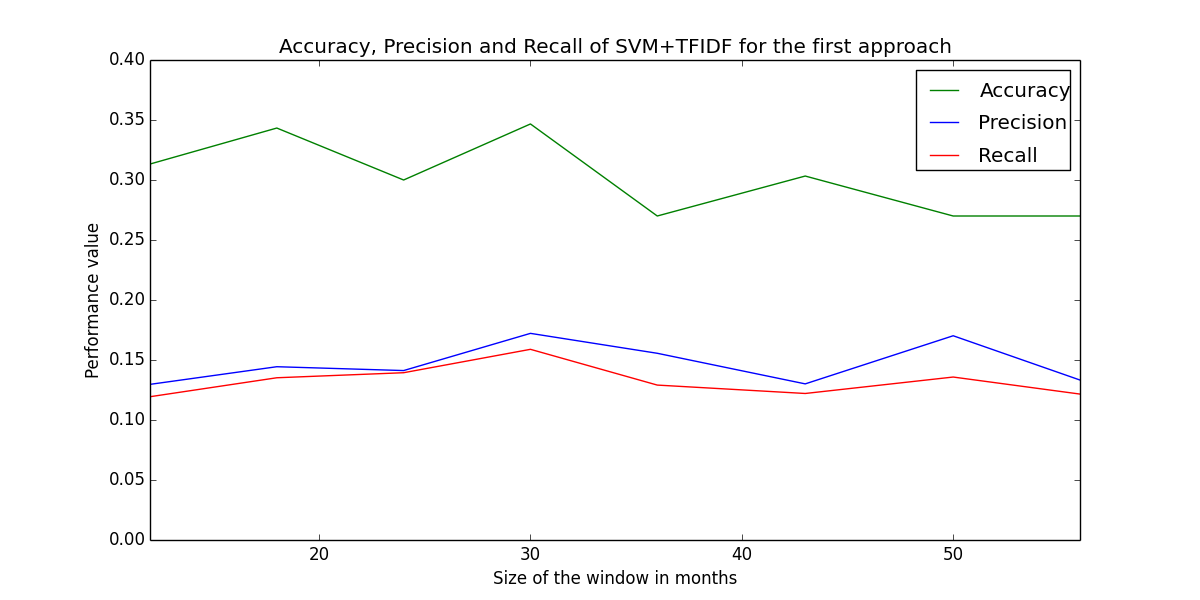
\includegraphics[width=\textwidth]{./images/window_size/firefox_1a.png}
    \caption{Performance of the classifier for different size of the window, 1st approach}
    \label{fig:window.firefox.1a}
\end{figure}

\subsection{Second Approach}

In the second approach, we employ the same periods, except period 1 that is about 15 months long. Another difference is that each train set contains 3000 randomly selected bug reports from period 1, 1-2, 1-3 etc. and the size of the sample is in this case therefore fixed, what is different is the period from which they were selected. From each bin, all bug reports that were fixed by a developer with less than 30 fixed bugs within the same train set are removed. We also remove all bug reports from cross-validation set that are not in the train set. We do this to get more relevant results from macro-averaged metrics, because otherwise the result of such metrics would be very close to zero.

The disadvantage of the second approach is that it does not really tell us what size of the window can be used to get the best performance. What it shows is whether the size of the window from which an equal size of sample is selected matters.

Figure~\ref{fig:window.firefox.2a} shows the plot of this approach. The performance decreases as the size of the window increases, which is expected. Precision and recall however increases when the size of the window is around 45 months.~\todo{Try to figure out why}

\begin{figure}[htbp]
    \centering
        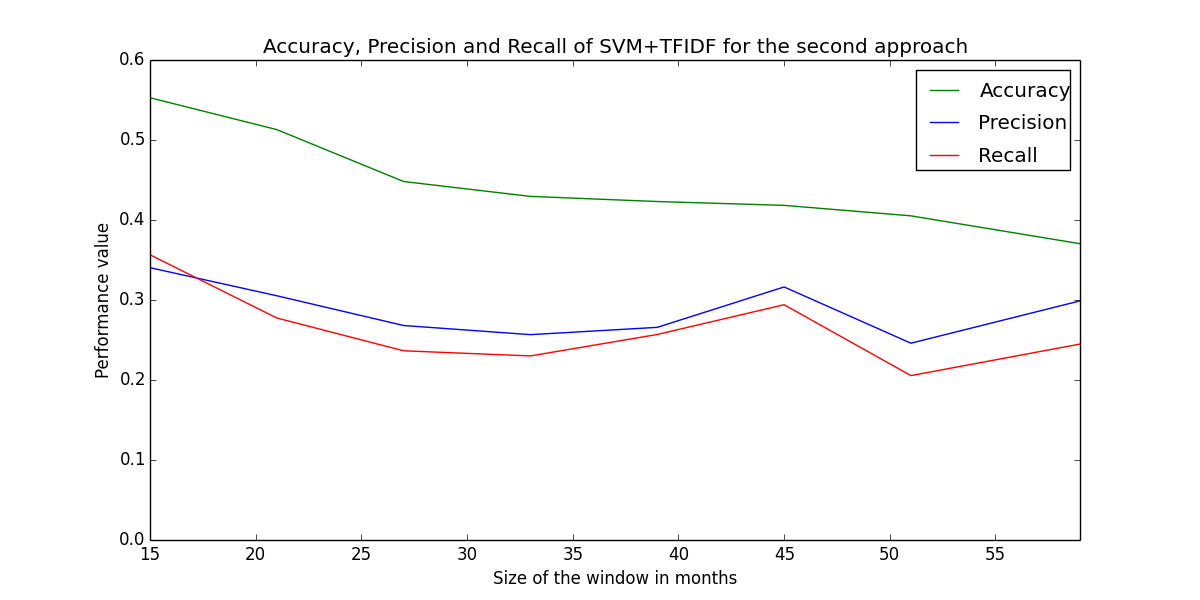
\includegraphics[width=\textwidth]{./images/window_size/firefox_2a.png}
    \caption{Performance of the classifier for different size of the window, 2nd approach}
    \label{fig:window.firefox.2a}
\end{figure}

\subsection{Third Approach}

Finally, in the third approach, we again use the same periods as in the second approach. The difference is that we select all bug reports as train set.

The advantage is that this approach is that it is closest to reality (no random selection). The disadvantage is, however, that the results are skewed by a variable number of samples in each period. The last major disadvantage is that the number of classes (developers) increases significantly each time samples from another period are added.

TODO: Add the plot of this approach and write about it (takes a lot of time to train SVM on 9000 data samples...).

\section{Baseline}

In this section, we establish a baseline for our models. Our baseline is very simple, the number of bug report that is assigned to each developer is counted and the developer with highest number of reports is selected as a prediction for each subsequent call of the \texttt{predict} function.

Figure~\ref{fig:models.firefox.stopwords} shows the performance of the baseline model on Firefox data. While the accuracy of this model is relatively high (18\%), the precision and recall values are much lower (1\% and 5\%), which can be explained by the way macro-averaged metrics work, see TODO\todo{Replace with reference to the chapter/section which describes the metrics}. 

\section{Stop-Words Removal}

Stop-words removal is a technique that can increases performance of the model. In this section, we determine whether the increase is significant enough to use it for subsequent comparisons of models.

Figure~\ref{fig:models.firefox.stopwords} shows the increase in performance after all stop-words were removed from the feature vector of the Firefox data. You can see that the performance of the classifier slightly increased on all models. Accuracy increased by 3\%, 0\% and 1\% on SVM, Naive Bayes and CART model respectively. Precision value of the SVM model decreased by 1\% but increased by 6\% with Naive Bayes and by 1\% with CART. Finally, Recall values of SVM and Naive Bayes increased by 4\% and 2\% respectively while it slightly decreased on the CART model by about 1\%.

\begin{figure}[htbp]
    \centering
        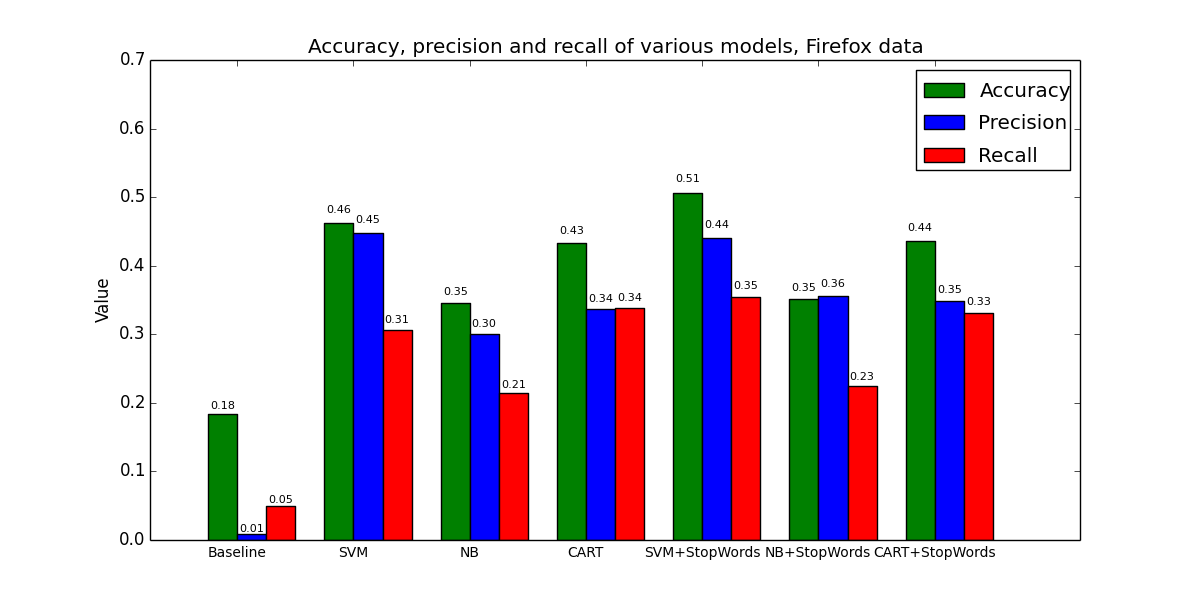
\includegraphics[width=\textwidth]{./images/comparison_of_models/firefox_0.png}
    \caption{Stop-Words removal on Firefox data.}
    \label{fig:models.firefox.stopwords}
\end{figure}

The results of the other datasets were similar in nature. We therefore conclude that the performance boost of stop-words removal is significant enough to warrant better results, which matches the conclusion of Čubranić and Murphy~\cite{Murphy} (see chapter~\ref{chapter:related-work}). Thus, in our evaluation, we always use stop-words removal in combination with other feature extraction/selection methods.

\section{Comparison of Models}

In the following text, comparison of the models is presented. We show the accuracy, precision and recall of these models on three datasets.\todo{What models? Explain or provide reference.}\todo{Explanation of these measurement metrics should be somewhere and perhaps a reference would be in order.} This comparison allows us to conclude what model is best for this application.

\subsection{Firefox Data}

On Figure~\ref{fig:results.models.firefox}, you can see the performance of the chosen models on Firefox data. The SVM model with TF-IDF weighing achieves the best performance with accuracy of 57\%. It's precision and recall also outperforms all the other approaches with values of 51\% and 45\%. The same model with LSI takes second place. The only model other than SVM that approaches SVM with it's performance is CART, especially with TF-IDF weighing.

\begin{figure}[htbp]
    \centering
        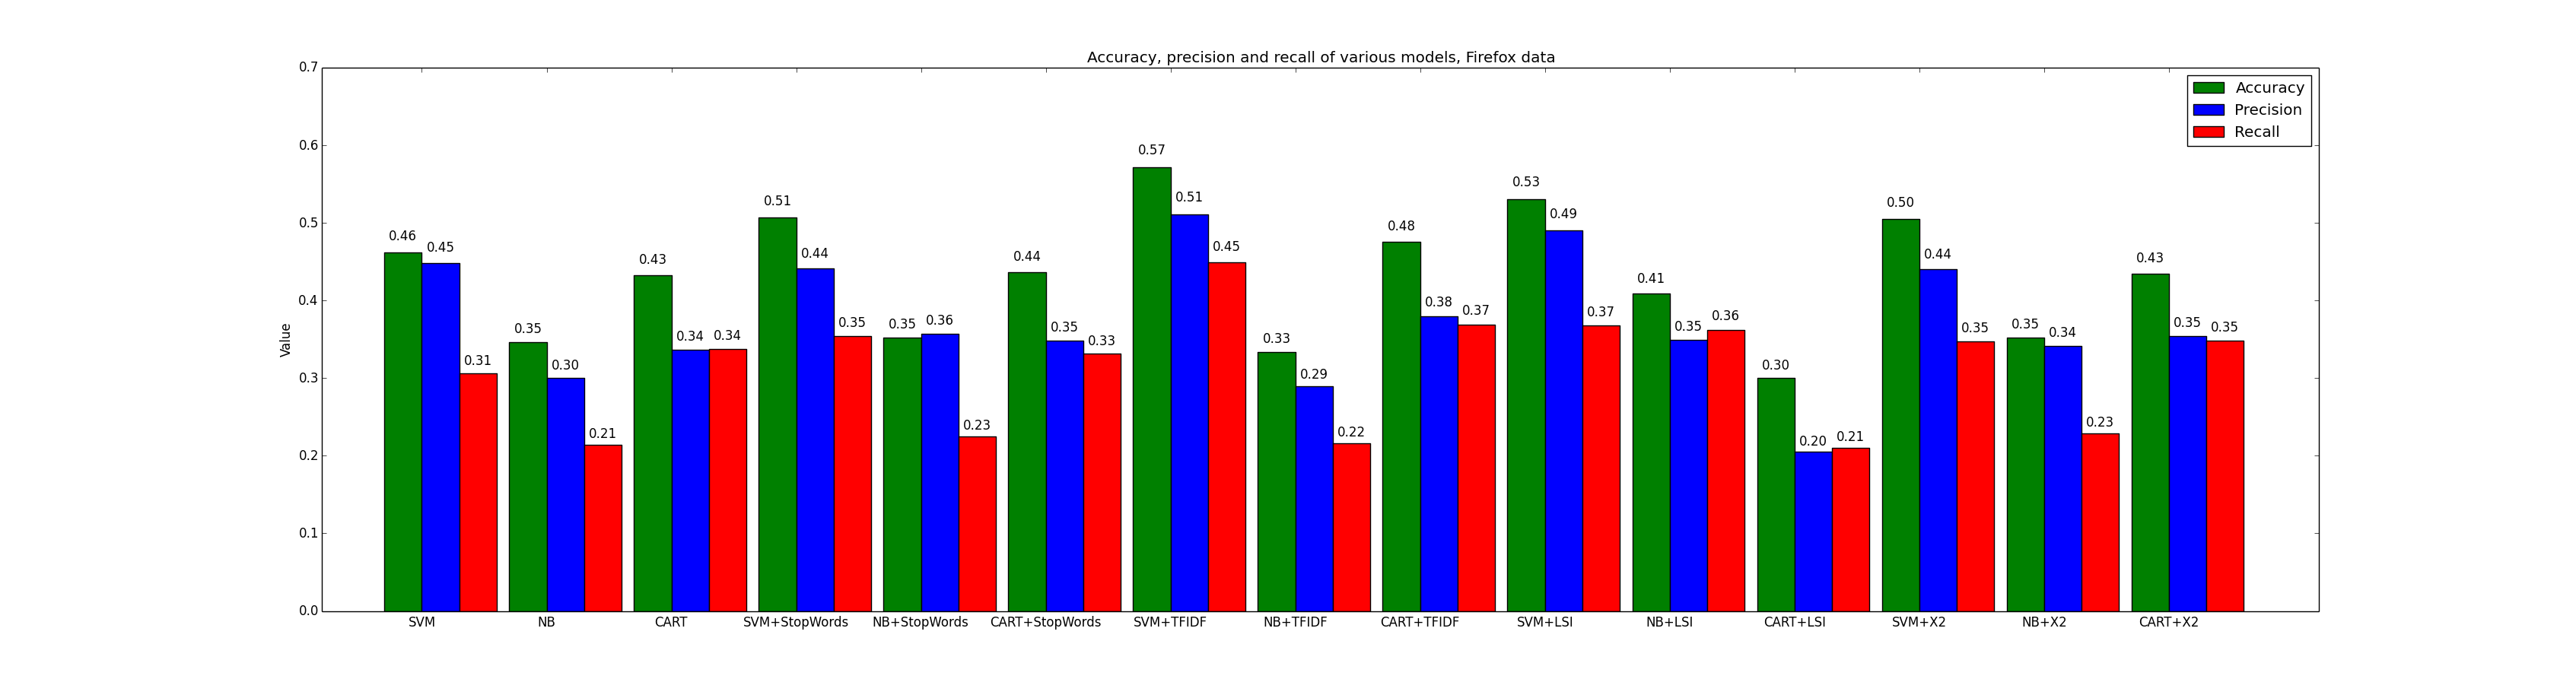
\includegraphics[width=\textwidth]{./images/comparison_of_models/firefox.png}
    \caption{Comparison of models on Firefox data.}
    \label{fig:results.models.firefox}
\end{figure}

\subsection{Netbeans Data}

The performance of the models on Netbeans data is shown on Figure~\ref{fig:results.models.netbeans}. It is clear that the SVM model with TF-IDF weighing performs best even on the Netbeans data, although in this case the LSI feature extraction technique does not seem to perform as well as in the previous case. The accuracy, precision and recall of the approach are 53\%, 53\% and 49\% respectively. Sole SVM model and SVM+$\chi^2$ model perform similarly as far as precision is concerned, while the accuracy and recall values are lagging behind by a considerable margin. None of the other models offer better performance than even sole SVM model on this data, which suggests that SVM is a very good choice in this domain.

\begin{figure}[htbp]
    \centering
        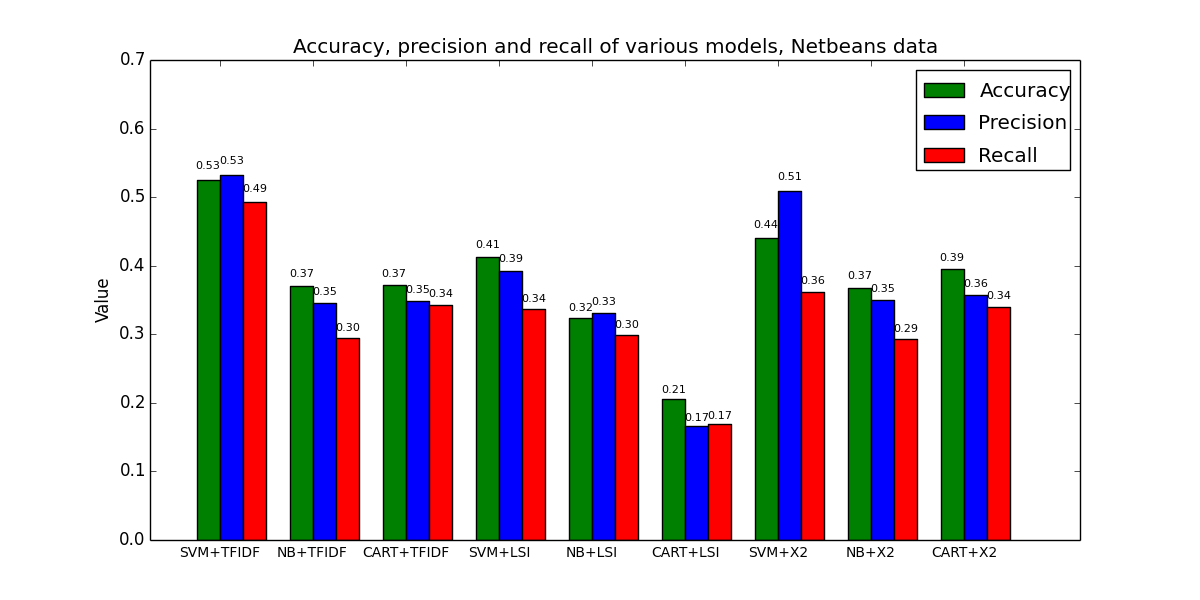
\includegraphics[width=\textwidth]{./images/comparison_of_models/netbeans.png}
    \caption{Comparison of models on Netbeans data.}
    \label{fig:results.models.netbeans}
\end{figure}

\subsection{Proprietary Data}

In this case, the performance of all models decreased a lot in comparison with the other datasets. However, even in this case, the SVM model with TF-IDF offers the best performance of 37\% accuracy, 32\% precision and 31\% recall. The same model with LSI also shows quite a good performance and quite surprisingly, the Naive Bayes model with LSI performs quite well as far as precision and recall is concerned. Figure~\ref{fig:results.models.proprietary} presents the results in graphical manner.

\begin{figure}[htbp]
    \centering
        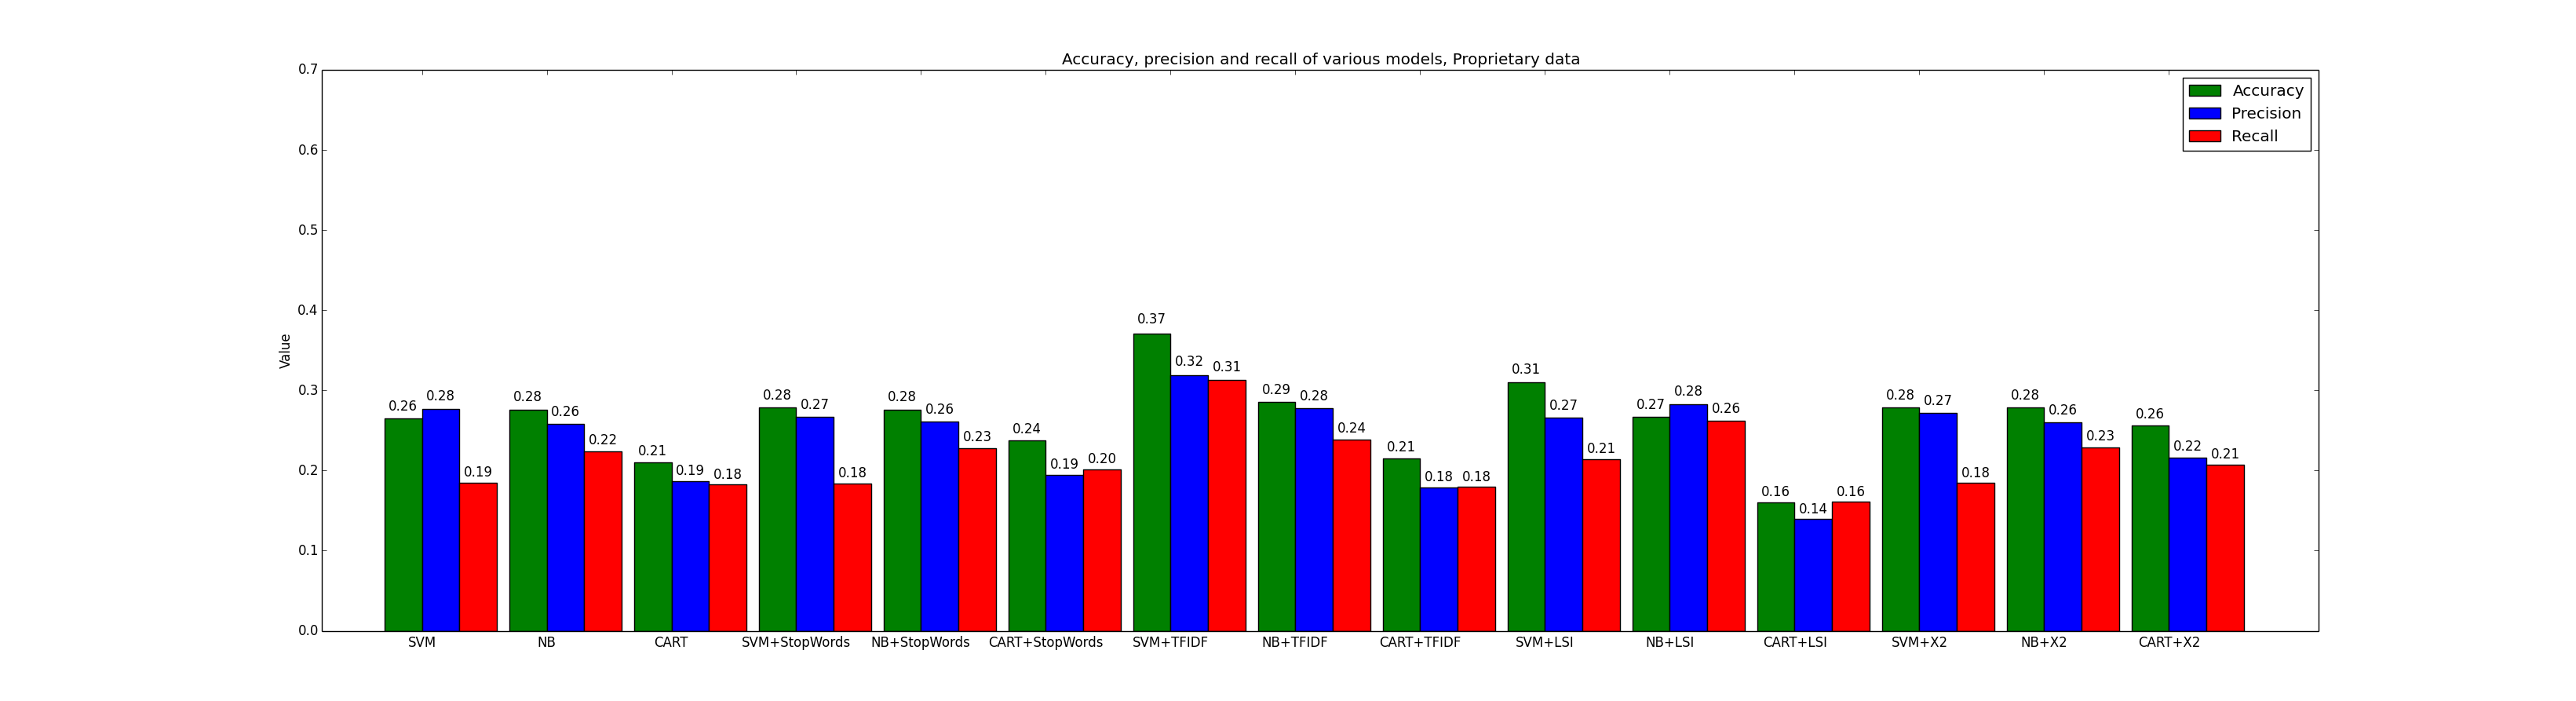
\includegraphics[width=\textwidth]{./images/comparison_of_models/proprietary.png}
    \caption{Comparison of models on the Proprietary data.}
    \label{fig:results.models.proprietary}
\end{figure}

\subsection{Conclusion}

The comparison shows that SVM with TF-IDF weighing performs best on all datasets. Not only that, it also generalizes very well, because there was no need to readjust the parameters of the model to get the best or nearly the best performance for all datasets. The disadvantage of the model is that it is the most computationally complex one, because SVM is the slowest of the three models, there are a lot of classes and there are a lot of features. This can be at least partially dealt with by using $\chi^2$ feature extraction in conjunction with TF-IDF while sacrificing some of the performance.

\section{Comparison of Datasets}

The main purpose of this section is to compare proprietary dataset with open-source dataset. The open-source dataset used for this is from the Firefox project. We selected equal number of reports from both datasets to construct an accurate comparison.\todo{Maybe it would be useful to compare with the Netbeans data too.}\todo{And also it could be quite interesting to use the CART model too.}

\subsection{Naive Bayes Model}

The first model for comparison is Naive Bayes. The only used feature extraction method for this model is stop-words removal.

First plot (Figure \ref{fig:results.datasets.nb_accuracy}) represents accuracy of the Naive Bayes model. You can already see that the open source data perform better than the proprietary data. Accuracy of the classifier is 35\% vs 24\% when $x$ (see above) is set to 30. In the following text, we will always compare the results of this setting of parameter $x$ as we believe that is the best production value for the given size of the dataset.

\begin{figure}[htbp]
    \centering
        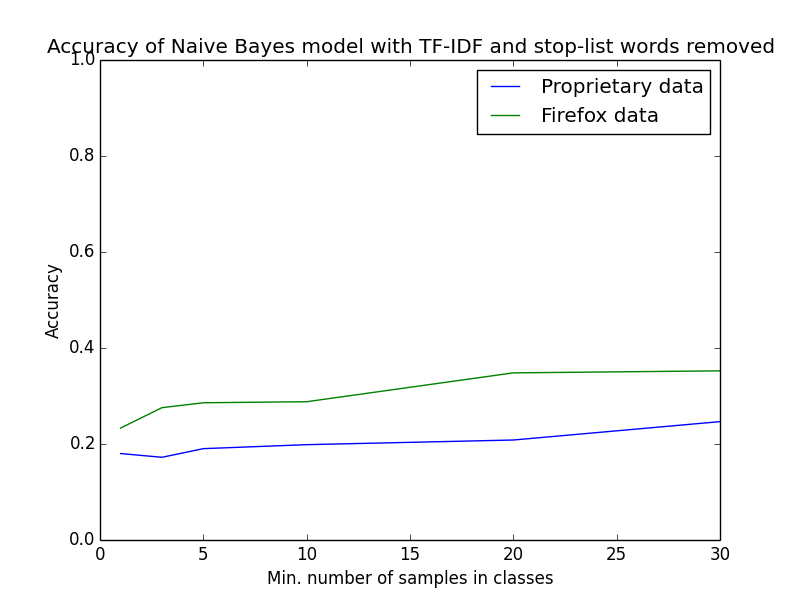
\includegraphics[width=\textwidth]{./images/prop_vs_os/nb_accuracy.png}
    \caption{Comparison of accuracy of Naive Bayes model.}
    \label{fig:results.datasets.nb_accuracy}
\end{figure}

Second plot (Figure \ref{fig:results.datasets.nb_pr}) is a representation of precision and recall of the same model. Precision of the classifier is 46\% and 22\% for the open source and proprietary data, respectively. Recall value is 29\% for the open source data and 19\% for the proprietary data.

\begin{figure}[htbp]
    \centering
        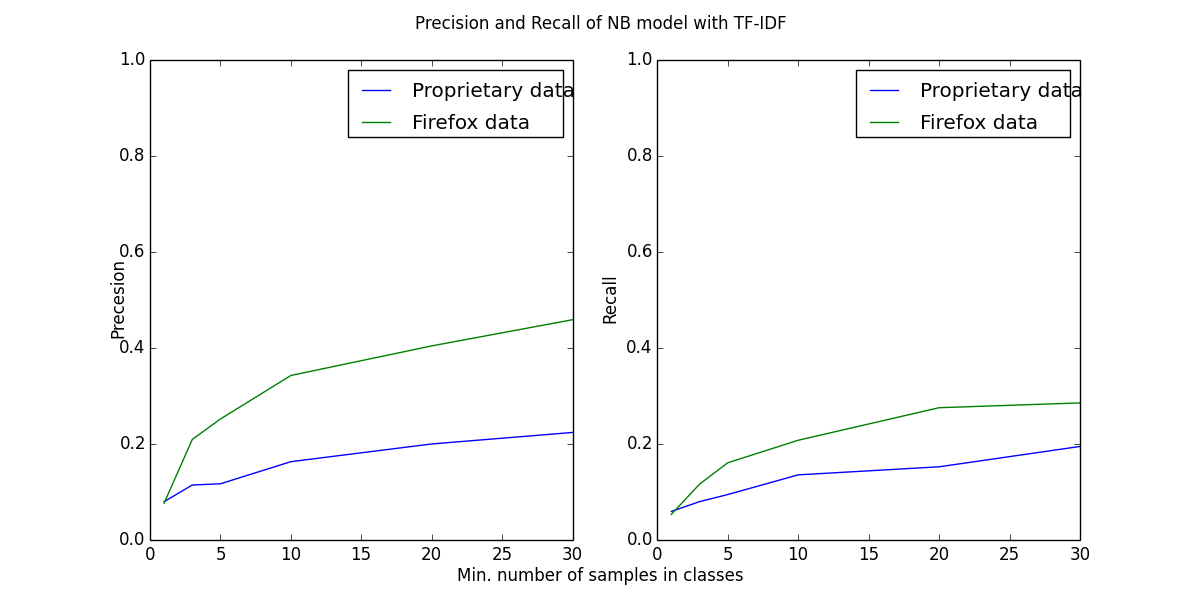
\includegraphics[width=\textwidth]{./images/prop_vs_os/nb_precision_and_recall.png}
    \caption{Comparison of precision and recall of Naive Bayes model.}
    \label{fig:results.datasets.nb_pr}
\end{figure}

\subsection{Support Vector Machine Model}

The second model used for comparison of the proprietary dataset with the open-source dataset is Support Vector Machine model with TF-IDF weighing and stop-words removal as this model shows the most promising results.

Figure \ref{fig:results.datasets.svm_accuracy} visualizes accuracy of the model. Even with this model, the open source data perform much better with accuracy value of 54\% vs 33\% of the proprietary data.

\begin{figure}[htbp]
    \centering
        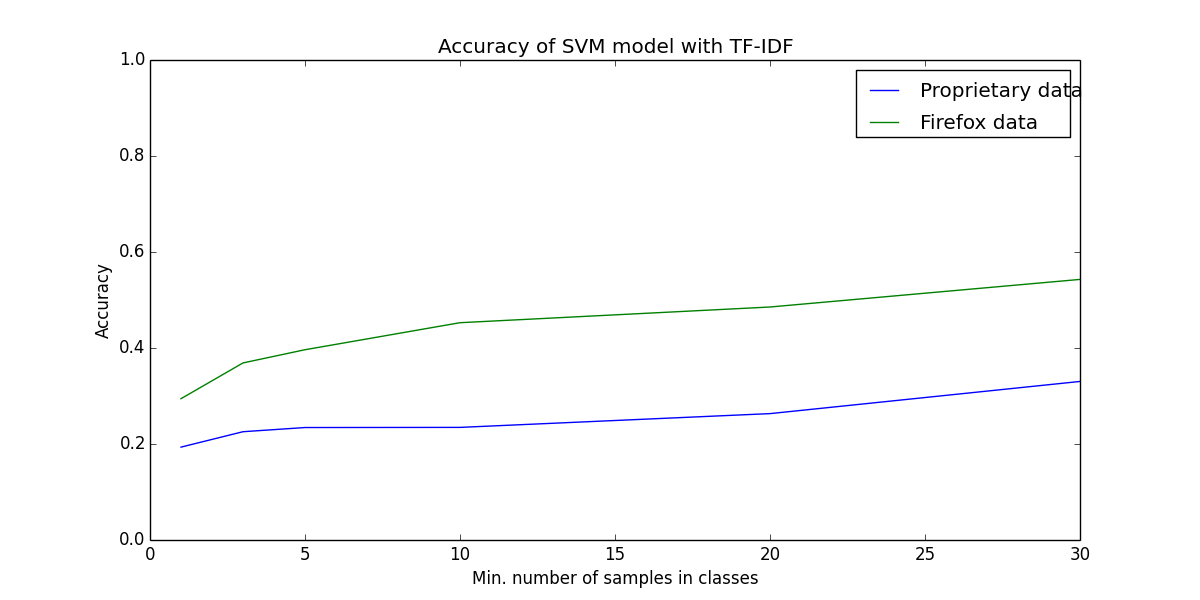
\includegraphics[width=\textwidth]{./images/prop_vs_os/svm_accuracy.png}
    \caption{Comparison of accuracy of SVM model.}
    \label{fig:results.datasets.svm_accuracy}
\end{figure}

Precision and recall of the SVM model is pictured on figure \ref{fig:results.datasets.svm_pr}. It again clearly shows that the precision value of the open source data is higher (again about 54 \%) than the precision value of the proprietary data (32\%). The recall value is 49\% for the open-source data and 26\% for the proprietary data.

\begin{figure}[htbp]
    \centering
        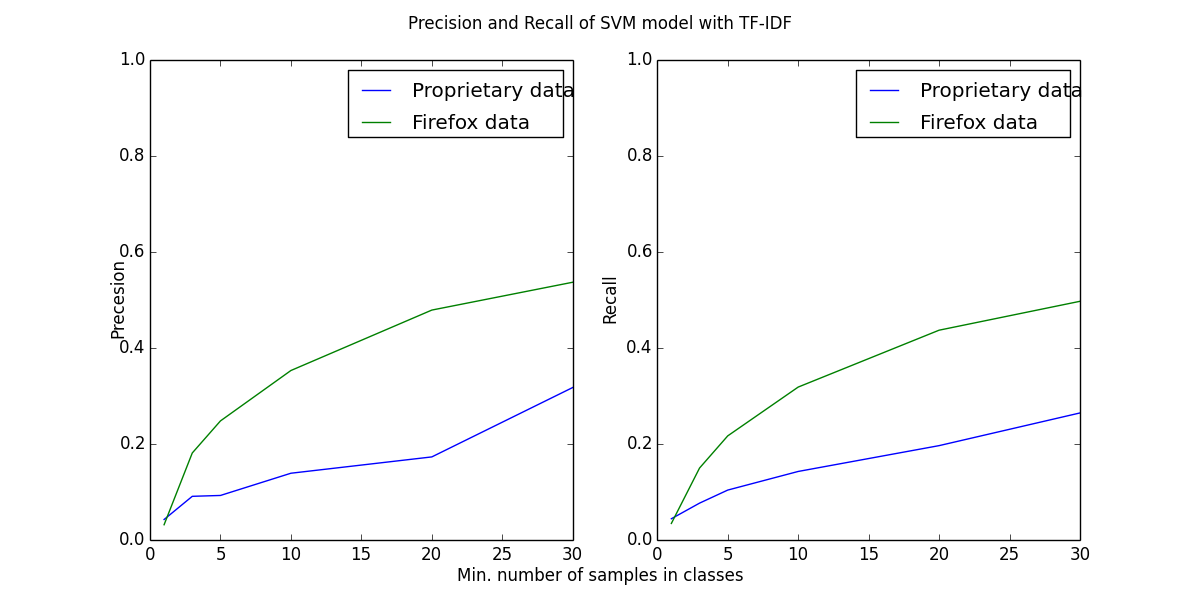
\includegraphics[width=\textwidth]{./images/prop_vs_os/svm_precision_and_recall.png}
    \caption{Comparison of precision of SVM model.}
    \label{fig:results.datasets.svm_pr}
\end{figure}

\subsection{Conclusion}

The results clearly show that the open-source data provide much better performance. The number of classes is very similar and the number of reports used for training too, so it is clear that the quality of the open-source reports is higher.\todo{Or maybe there is something else? Try to figure out if that is really the case, if it is, it might be better to provide a better explanation.}

\section{Comparison of Performance for Variable Number of Recommendations}

We look at the performance of the models for different number of recommendations in this section. The plots will show the performance for number of recommendations from 1 to 10.\todo{More than one model might be in order.}

\subsection{Support Vector Machine Model}

For this comparison, we, again, take the SVM model with TF-IDF weighing and stop-words removed. Figure \ref{fig:results.topx.svm_accuracy} shows how the accuracy increases when the number of recommendations increases, which is expected as the more there are recommendation, the higher the chance of a hit is.\todo{Precision and recall would be useful too maybe.}

\begin{figure}[htbp]
    \centering
        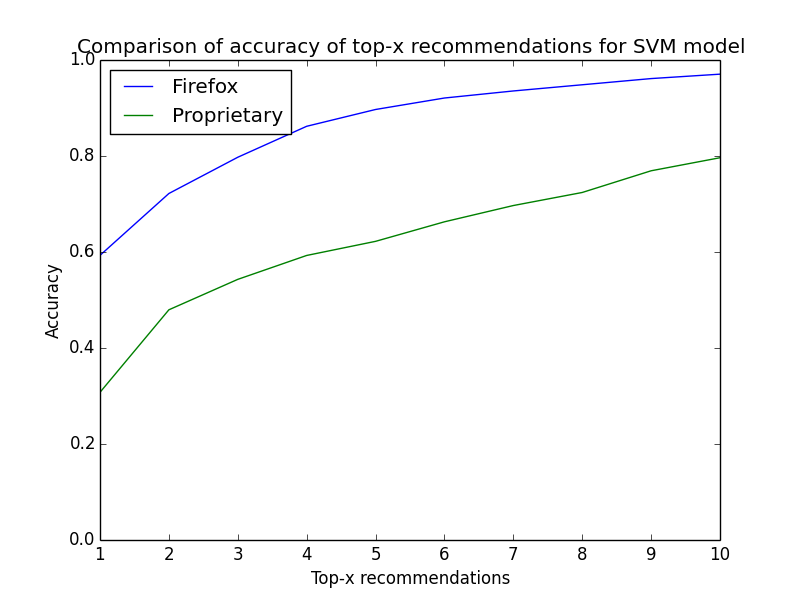
\includegraphics[width=250px]{./images/top_x_comparison/svm_accuracy.png}
    \caption{Comparison of accuracy of top-x recommendations for SVM model.}
    \label{fig:results.topx.svm_accuracy}
\end{figure}

It is apparent from the plot that the highest performance boost happens when the number of recommendations changes from one to two both for the proprietary data and the Firefox data. 

\subsection{Conclusion}

From the results in this section, we concluded that the best number of recommendations to suggest to users is 5. The performance does not increase very much with more recommendations and it would probably only lead to confusion if the number of recommendations was too high.